Dado el siguiente problema de probramación lineal:


\begin{equation}
\begin{split}
\mbox{max. } z = 3x_1 + 2x_2\\
s.a.:\\
x_1 + 2x_2 \leq 60\\
x_1 + x_2 \geq 10\\
x_1 \leq 30\\
x_1,\,\,x_2\geq 0\\
\end{split}
\end{equation}

Se pide identificar una solución de cada uno de los siguientes tipos explicando por qué cumple con lo que se indica:
\begin{enumerate}
    \item Tipo 1: solución no básica y factible.
    \item Tipo 2: solución básica y factible.
    \item Tipo 3: solución básica y no factible.
    \item Tipo 4: solución no básica y no factible.
    \item ¿Cuál de los cuatro tipos de soluciones anteriores cumple que sus soluciones siempre ofrecen mejores valores de la función objetivo que las de cualesquiera otro de los tipos?
    \item Indica y justifica un valor que sea cota inferior del problema dual (\ref{ec:4}).

\end{enumerate}

Reformulamos el problema en forma estándar:

\begin{equation}
\begin{split}
\mbox{max. } z = 3x_1 + 2x_2\\
s.a.:\\
x_1 + 2x_2 + h_1 = 60\\
x_1 + x_2 - h_2 = 10\\
x_1 + h_3 = 30\\
x_1,\,\,x_2,\,\,h_1,\,\,h_2,\,\,h_3\geq 0\\
\end{split}
\end{equation}

Podemos representar gráficamente el problema para facilitar la tarea:

\begin{center}
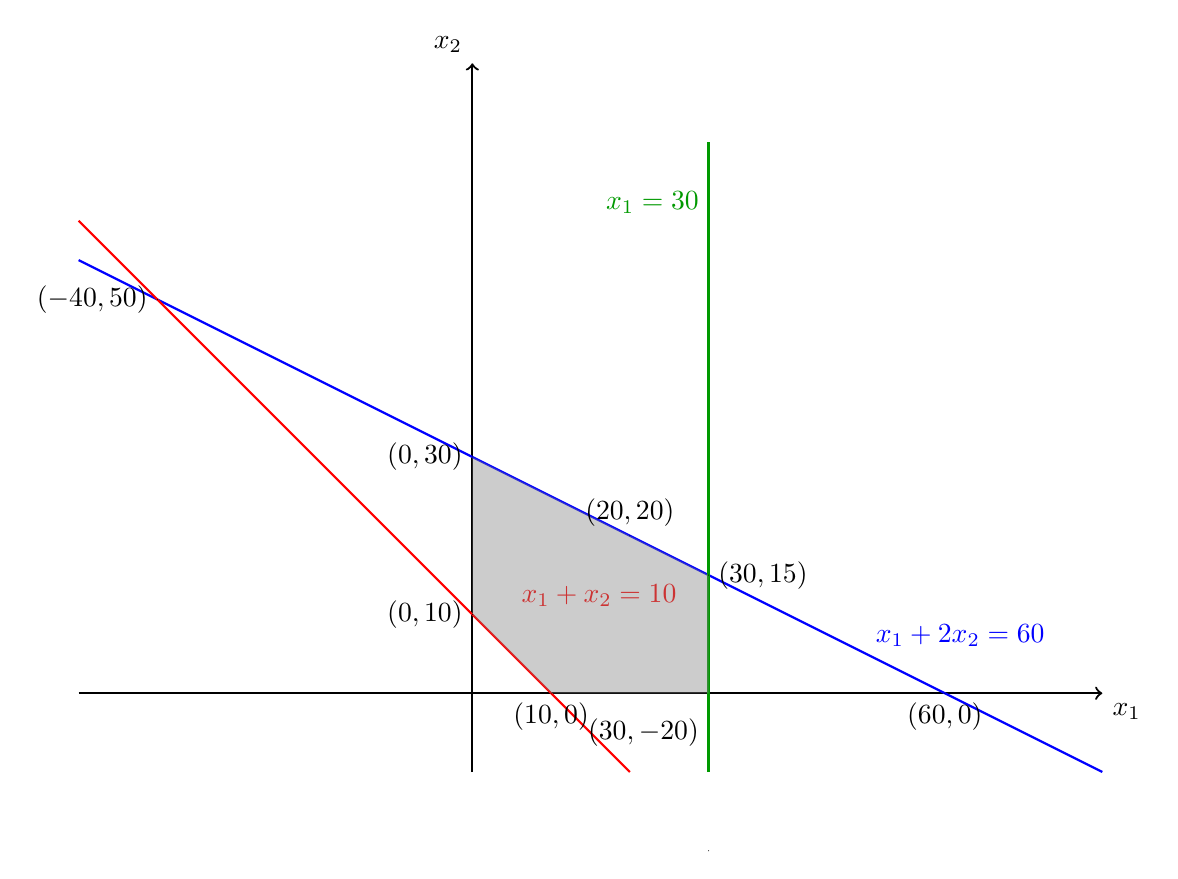
\begin{tikzpicture}[scale=0.1]

% Ejes coordenados
\draw[thick,->] (-50,0) -- (80,0) node[anchor=north west] {$x_1$};
\draw[thick,->] (0,-10) -- (0,80) node[anchor=south east] {$x_2$};

% Restricción 1: x1 + 2x2 <= 60
\draw[thick,blue] (-50,55) -- (80,-10);
\node[blue,anchor=north west] at (50,10) {$x_1 + 2x_2 = 60$};

% Restricción 2: x1 + x2 >= 10
\draw[thick,red] (-50,60) -- (20,-10);
\node[red,anchor=north west] at (5,15) {$x_1 + x_2 = 10$};

% Restricción 3: x1 <= 30
\draw[thick,green!60!black] (30,-10) -- (30,70);
\node[green!60!black,anchor=north east] at (30,65) {$x_1 = 30$};

% Región factible
\fill[gray,opacity=0.4] (10,0) -- (0, 10) -- (0,30) -- (30,15) -- (30,0);

% Intersecciones dentro y fuera de la región factible
% Intersección 1: x1 + 2x2 = 60 y x1 + x2 = 10
\fill[black] (20,20) circle (2pt);
\node[anchor=south] at (20,20) {$(20,20)$};

% Intersección 2: x1 + 2x2 = 60 y x1 = 30
\fill[black] (30,15) circle (2pt);
\node[anchor=west] at (30,15) {$(30,15)$};

% Intersección 3: x1 + x2 = 10 y x1 = 30
\fill[black] (30,-20) circle (2pt);
\node[anchor=east] at (30,-5) {$(30,-20)$};

% Intersección 4: x1 + 2x2 = 60 y eje x2
\fill[black] (60,0) circle (2pt);
\node[anchor=north] at (60,0) {$(60,0)$};

% Intersección 5: x1 + x2 = 10 y eje x2
\fill[black] (10,0) circle (2pt);
\node[anchor=north] at (10,0) {$(10,0)$};

% Intersección 6: x1 + x2 = 10 y eje x1
\fill[black] (0,10) circle (2pt);
\node[anchor=east] at (0,10) {$(0,10)$};

% Intersección 7: x1 + 2x2 = 60 y eje x1
\fill[black] (0,30) circle (2pt);
\node[anchor=east] at (0,30) {$(0,30)$};

% Intersección 8: x1 + 2x2 = 60 y eje x1
\fill[black] (-40,50) circle (2pt);
\node[anchor=east] at (-40,50) {$(-40,50)$};

\end{tikzpicture}
\end{center}


\begin{enumerate}
    \item \textbf{Tipo 1: solución no básica y factible.}
    La solución donde $x_1 = 10$ y $x_2=1$ es no básica y factible porque:
    \begin{itemize}
        \item $h_1>0$, la solución no está sobre la restricción 1 y cumple dicha restricción.
        \item $h_2>0$, la solución no está sobre la restricción 1 y cumple dicha restricción.
        \item $h_3>0$, la solución no está sobre la restricción 3 y cumple dicha restricción.
    \end{itemize}
    La solución tiene cinco componentes no nulas (más que restricciones) así que es no básica y no se incumple ninguna restricción y satisface las restricciones de no negatividad, así que es factible.
    \item \textbf{Tipo 2: solución básica y factible.}
    La solución donde $x_1 = 10$ y $x_2=0$ es básica y factible porque:
    \begin{itemize}
        \item $h_1>0$, la solución no está sobre la restricción 1 y cumple dicha restricción.
        \item $h_2=0$, la solución está sobre la restricción 2.
        \item $h_3>0$, la solución no está sobre la restricción 3 y cumple dicha restricción.
    \end{itemize}
    
    La solución tiene tres componentes no nulas, es básica, no se incumple ninguna restricción y satisface las restricciones de no negatividad, es factible.
    \item \textbf{Tipo 3: solución básica y no factible.}
        La solución donde $x_1 = -40 < 0$ y $x_2=50$ es básica y no factible porque:
    \begin{itemize}
        \item $h_1=0$, la solución está sobre la restricción 1.
        \item $h_2=0$, la solución está sobre la restricción 2.
        \item $h_3>0$, la solución no está sobre la restricción 3 y cumple dicha restricción.
    \end{itemize}
    La solución tiene tres componentes no nulas, es básica, y se incumplen  las restricciones de no negatividad, es no factible.

    \textcolor{red}{\textbf{Error frecuente} \\
    Elegir tres variables y asignarles valor diferente de cero -alguno negativo- y el asignar al resto de variables valor nulo.\\
    Si se eligen tres variables como no nulas y el resto nulas, las tres primeras deben corresponder a una base y, por lo tanto, deben tener los valores resultantes de resolver las ecuaciones cuando se eliminan las variables no básicas.\\
    Por ejemplo, una solución del tipo $x^T=\begin{array}{ccccc}(-100 & -100 & -5 & 0 & 0)\end{array}$ no es básica porque cuando se seleccionan como variables básicas $x_1$, $x_2$ y $h_1$, es decir, si $h_2=h_3=0$, los valores de $x_1$, $x_2$ y $h_1$ no son, respectivamente -100, -100 y -5.}
    
    \item \textbf{Tipo 4: solución no básica y no factible.}
    La solución donde $x_1 = -1 < 0$ y $x_2=-1$ es básica y no factible porque:
    \begin{itemize}
        \item $h_1>0$, la solución no está sobre la restricción 1 y cumple dicha restricción.
        \item $h_2<0$, la solución no está sobre la restricción 3 y no cumple dicha restricción.
        \item $h_3>0$, la solución no está sobre la restricción 3 y cumple dicha restricción.
    \end{itemize}
    La solución tiene más de tres componentes no nulas, es no básica, y se incumple una restricción además de las restricciones de no negatividad, es no factible.
    \item \textbf{¿Cuál de los cuatro tipos de soluciones anteriores cumple que sus soluciones siempre ofrecen mejores valores de la función objetivo que las de cualesquiera otro de los tipos?}
    
    No se puede afirmar nada, porque no hay garantías de que toda las soluciones de un tipo tengan mejor función objetivo que los de las soluciones de otro tipo.

    \textcolor{red}{\textbf{Error frecuente} \\
    Ofrecer un conjunto de valores que no cumplen con las ecuaciones\\
    Indicar que la soluciones de tipo 2 son más interesantes que las restantes. En este apartado se preguntaba por el tipo de solución es siempre mejor que el resto y esto no ocurre para ninguna de ellas. Podemeos encontrar soluciones factibles y no básicas y con mejor función objetivo que otras básicas y factibles.\\    
    No se trata de enunciar lo que dice el teorema fundamental sino de responder a la pregunta específica que se hacía tal y como se indica.}

    \item \textbf{Un valor que sea cota inferior del problema dual de (P)}.
    
    El valor de la función objetivo de cualquier solución factible de (P) es cota inferior de su dual; por ejemplo 60 (valor de la función objetivo de la solución factible $x_1=0$, $x_2=30$).

\end{enumerate}